% Ejercicio 9, inciso a) — issue #1. Mismo contenido que inciso-a.md.
% Fragmento sin preámbulo: lo incluye latex/main.tex, que ya pone el título del inciso.

\begin{quote}
\itshape
Identifica el patrón de diseño más adecuado, justifica tu selección basándote en las
características del problema y explica la propuesta de solución considerando las clases
que intervienen y las relaciones entre ellas. ¿Por qué no usar Mediator o polling?
\end{quote}

\subsubsection{Patrón seleccionado: Observer (Publicador / Suscriptor)}

Observer define una dependencia uno-a-muchos entre objetos: cuando un objeto cambia de
estado, todos sus dependientes son notificados y se actualizan automáticamente
(Gamma et al., 1994, p.~326).

\subsubsection{Justificación}

El libro de la «banda de los cuatro» (\emph{Gang of Four}, GoF), la referencia clásica de
los patrones de diseño, recomienda Observer cuando un cambio en un objeto obliga a cambiar
otros y no se sabe
cuántos son, y cuando un objeto debe poder notificar a otros sin hacer suposiciones sobre
quiénes son (Gamma et al., 1994, pp.~327--328). Ambas condiciones se cumplen en este problema:

\begin{table}[H]
\centering
\small
\begin{tabularx}{\textwidth}{>{\raggedright\arraybackslash}X >{\raggedright\arraybackslash}X}
\toprule
\textbf{Característica del problema} & \textbf{Cómo la resuelve Observer} \\
\midrule
\textbf{Relación uno-a-muchos}: una acción, miles de clientes interesados.
  & El \emph{Sujeto} (la acción) mantiene una lista de \emph{Observadores} y les avisa a
    todos cuando cambia su precio. \\
\addlinespace
\textbf{No se sabe de antemano cuántos dependientes hay.} Los clientes eligen acciones y
umbrales y pueden cambiarlos en cualquier momento.
  & \texttt{Suscribir()} y \texttt{Desuscribir()} se llaman en tiempo de ejecución, sin
    tocar el código de la acción. \\
\addlinespace
\textbf{Notificación inmediata.}
  & El cambio de precio dispara \texttt{Notificar()} en ese mismo instante; el cliente no
    tiene que preguntar. \\
\addlinespace
\textbf{La acción no debe conocer a sus suscriptores} (bajo acoplamiento).
  & La acción solo conoce la interfaz \texttt{IObservadorPrecio}; no sabe si detrás hay un
    email, un SMS o un push. \\
\addlinespace
\textbf{Extensibilidad} (nuevos canales: WhatsApp, Telegram, webhook\ldots).
  & Se añade una nueva implementación de \texttt{ICanalNotificacion} sin modificar
    \texttt{Accion} (principio Abierto/Cerrado). \\
\bottomrule
\end{tabularx}
\caption{Características del problema y cómo las resuelve Observer.}
\end{table}

\begin{quote}
En .NET el patrón Observer viene incluso en la biblioteca base:
\texttt{IObservable<T>} / \texttt{IObserver<T>} y la palabra clave \texttt{event}. Aquí se
implementa de forma explícita para que se vean los roles del patrón.
\end{quote}

\subsubsection{Propuesta de solución: clases y relaciones}

\begin{figure}[H]
\centering
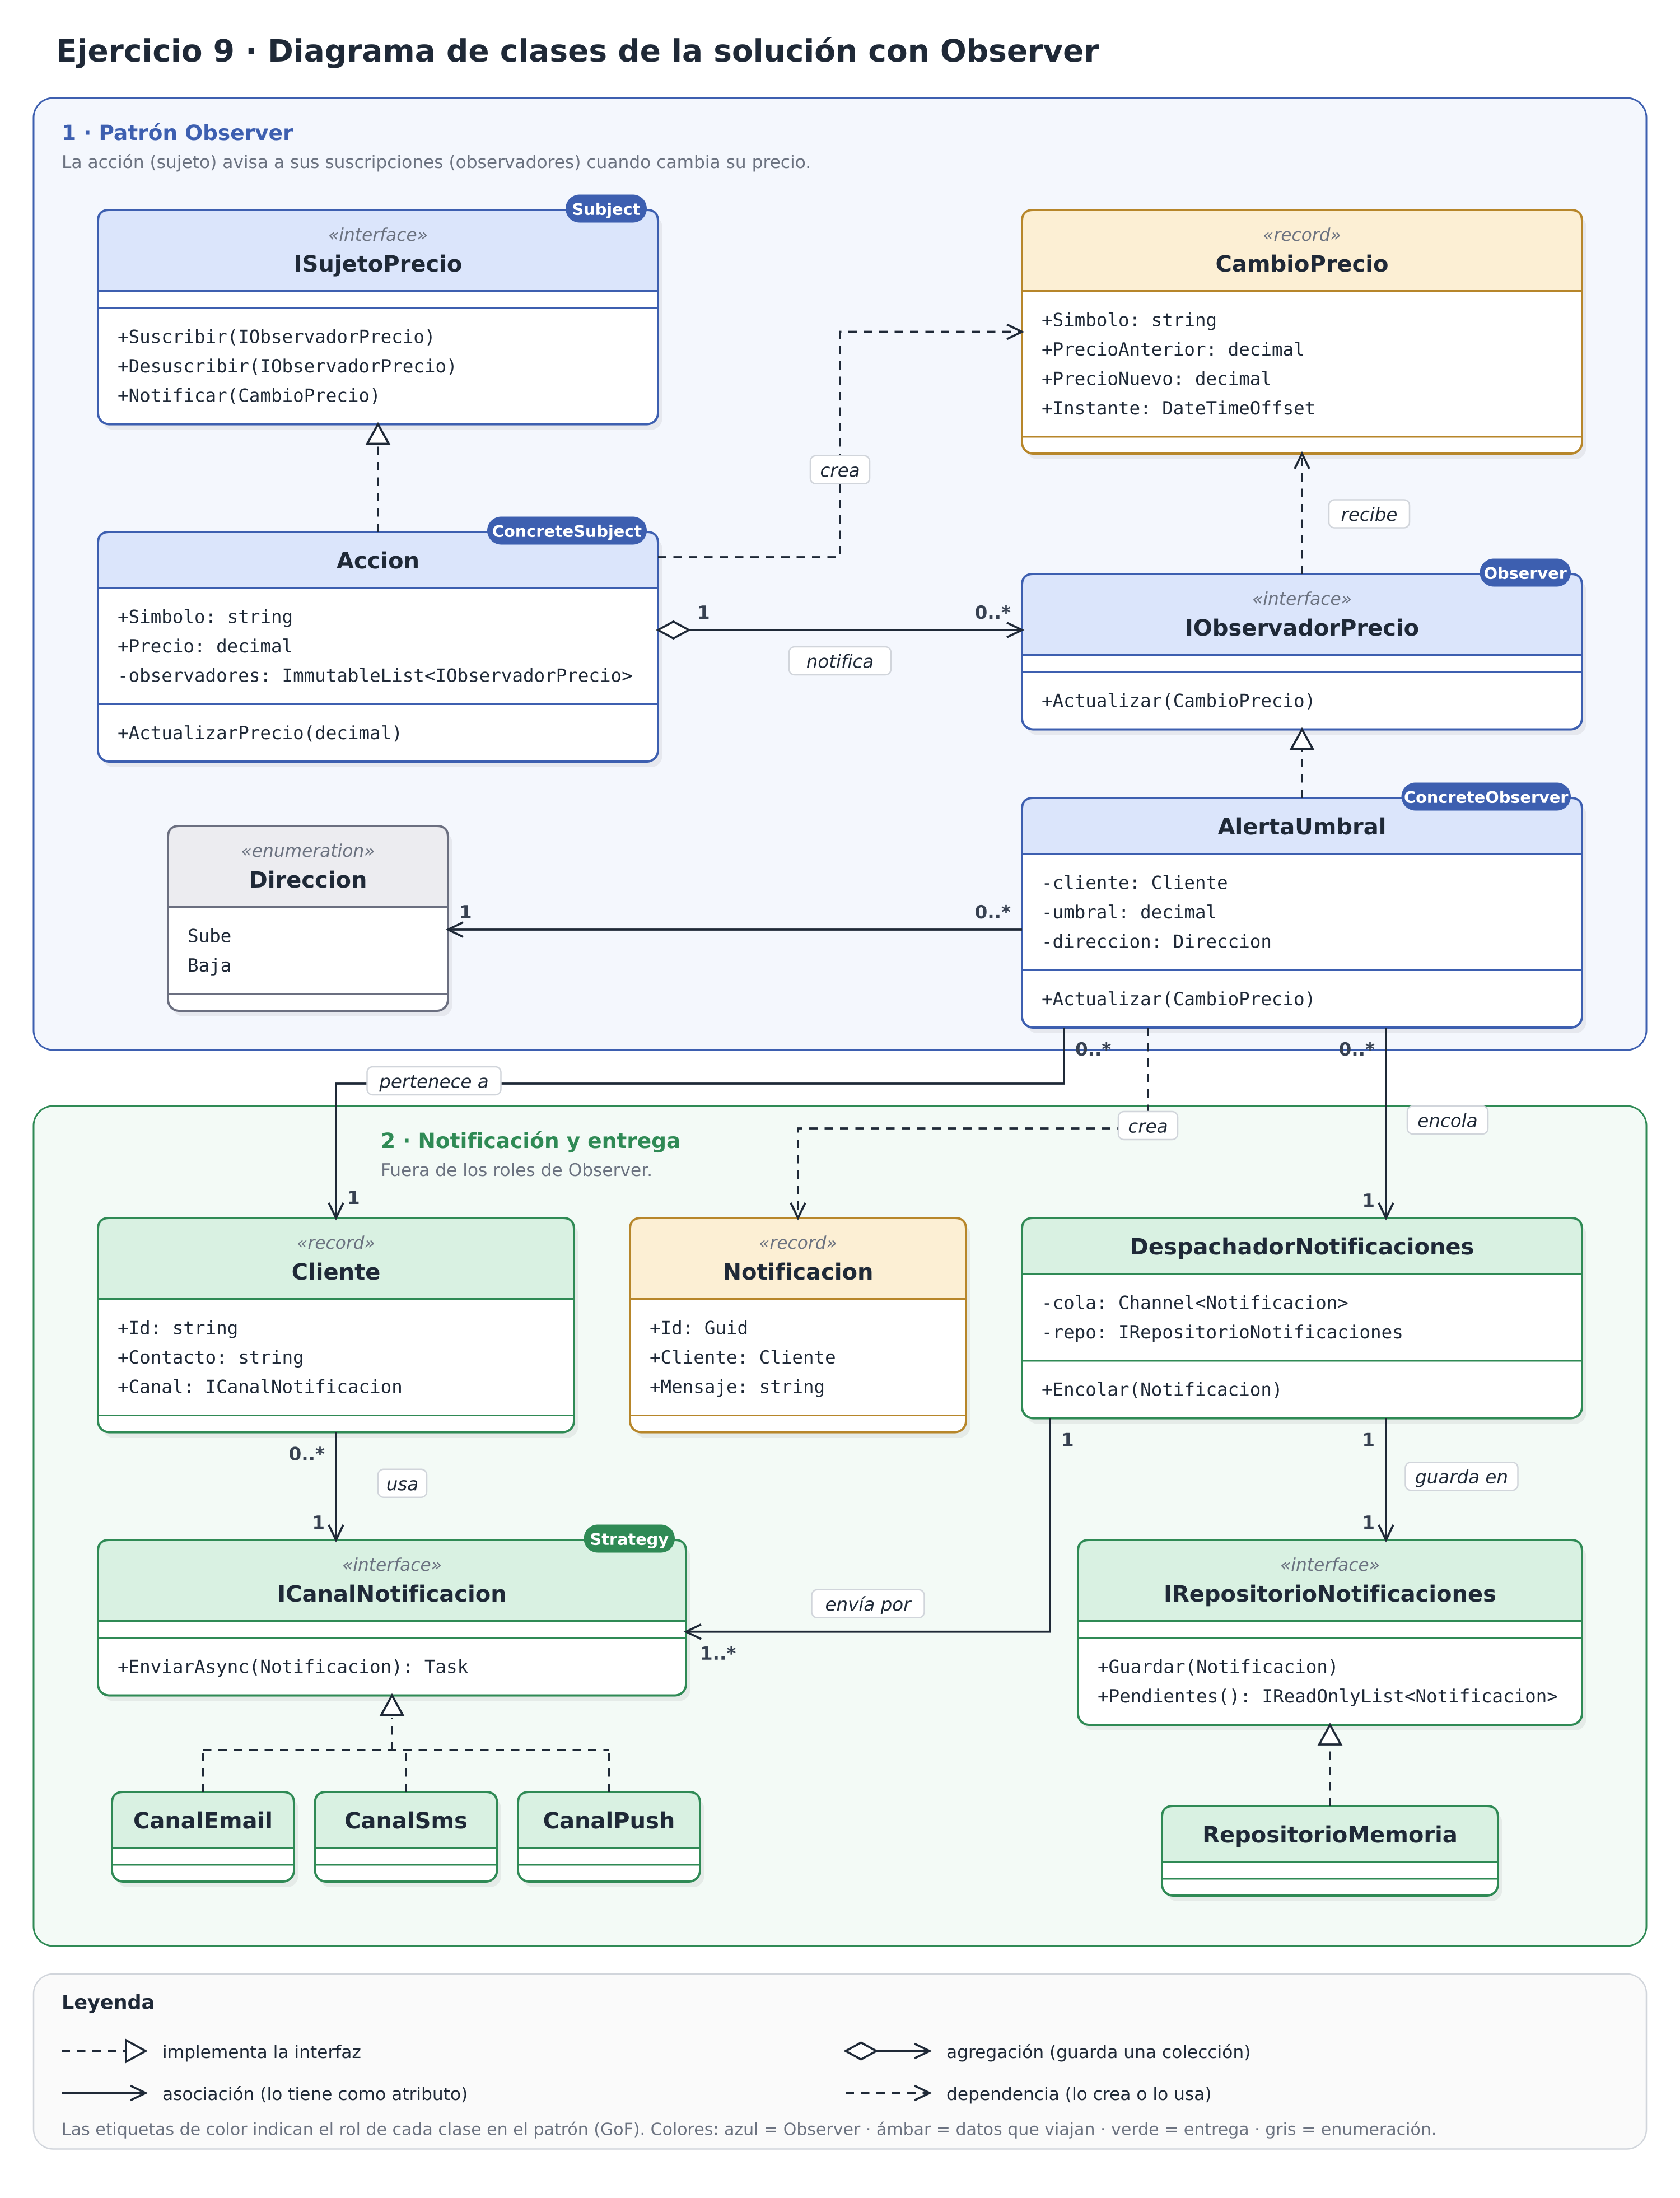
\includegraphics[width=0.92\textwidth]{ejercicio-09-notificaciones-bolsa/diagramas/inciso-a-clases.png}
\caption{Diagrama de clases UML de la solución con Observer.}
\label{fig:e9-clases}
\end{figure}

\paragraph{Roles del patrón.}
\begin{itemize}
  \item \textbf{Subject (\texttt{ISujetoPrecio})}: interfaz con \texttt{Suscribir},
        \texttt{Desuscribir} y \texttt{Notificar}.
  \item \textbf{ConcreteSubject (\texttt{Accion})}: guarda el símbolo y el precio. Cuando el
        precio cambia, crea un \texttt{CambioPrecio} y notifica a sus observadores. Una acción
        tiene de 0 a muchos observadores.
  \item \textbf{Observer (\texttt{IObservadorPrecio})}: interfaz con
        \texttt{Actualizar(CambioPrecio)}.
  \item \textbf{ConcreteObserver (\texttt{AlertaUmbral})}: representa \emph{una suscripción}
        de un cliente: acción, umbral y dirección (\texttt{Sube} o \texttt{Baja}). Decide si
        el cambio \textbf{cruza} su umbral y, si lo cruza, crea una \texttt{Notificacion}.
\end{itemize}

\paragraph{Clases de apoyo (fuera de los roles de Observer).}
\begin{itemize}
  \item \textbf{Canales (\texttt{CanalEmail}, \texttt{CanalSms}, \texttt{CanalPush})}: formas
        de envío intercambiables detrás de \texttt{ICanalNotificacion}. Funciona como un
        \textbf{Strategy}, porque cada cliente elige su canal. Los canales \textbf{no son
        observadores}: el observador decide \emph{si} hay que avisar, y el canal decide
        \emph{cómo} se entrega el aviso.
  \item \textbf{\texttt{DespachadorNotificaciones}}: separa la detección del evento del envío
        real. Se encarga de que el envío sea asíncrono (inciso c), de los reintentos y de la
        persistencia (restricción). En este inciso solo se presenta el diseño; se implementa
        en los incisos y en la restricción que lo usan. Guarda las notificaciones en un
        \texttt{IRepositorioNotificaciones}; \texttt{RepositorioMemoria} es la implementación
        en memoria que usa el inciso b.
\end{itemize}

\paragraph{Decisiones de diseño.}
\begin{itemize}
  \item \textbf{El observador es la suscripción (\texttt{AlertaUmbral}), no el
        \texttt{Cliente}.} Un cliente puede tener muchos umbrales sobre muchas acciones. Así
        cada observador tiene una sola responsabilidad: evaluar \emph{su} condición. El umbral
        vive dentro del observador, no en la acción, que no necesita saber qué le interesa a
        cada cliente.
  \item \textbf{Se notifica al cruzar el umbral.} Solo hay aviso cuando el precio
        \textbf{cruza} el umbral, no en cada \emph{tick} en que siga por encima. Así el cliente
        no recibe el mismo aviso una y otra vez.
\end{itemize}

\paragraph{Modelo push o pull.}
GoF distingue dos extremos. En el modelo \emph{push}, el sujeto envía a los observadores
información detallada del cambio, la necesiten o no. En el modelo \emph{pull}, el sujeto solo
avisa que algo cambió, y cada observador pide después lo que necesita
(Gamma et al., 1994, p.~332).

Esta solución usa el \textbf{modelo push}: \texttt{Notificar} envía un \texttt{CambioPrecio}
con el símbolo, el precio anterior y el nuevo. Hay dos razones:

\begin{enumerate}
  \item \textbf{Todos los observadores necesitan los mismos datos} (el precio anterior y el
        nuevo, para detectar el cruce). La desventaja que GoF señala para push, que el sujeto
        asume qué necesitan sus observadores, aquí no aplica.
  \item \textbf{Con pull, cada uno de los miles de observadores volvería a consultar a la
        acción} después de cada aviso. Eso es justo la ineficiencia que GoF atribuye a ese
        modelo (Gamma et al., 1994, p.~332), y además el precio podría haber cambiado otra vez
        entre el aviso y la consulta.
\end{enumerate}

\subsubsection{¿Por qué no usar Mediator?}

\begin{itemize}
  \item \textbf{Mediator resuelve otro problema.} Sirve para encapsular cómo interactúa un
        conjunto de objetos, y conviene cuando esos objetos se comunican ``de forma bien
        definida pero compleja'', con interdependencias desestructuradas
        (Gamma et al., 1994, pp.~305, 308). Un ejemplo es la comunicación muchos-a-muchos
        entre aviones del ejercicio~6. Aquí el flujo es \textbf{uno-a-muchos y en un solo
        sentido}: la acción emite y los clientes solo reciben. Los clientes nunca se
        comunican entre sí, así que no hay interacciones complejas que encapsular.
  \item \textbf{Un mediador central concentraría toda la lógica} en una sola clase: qué
        cliente quiere qué acción, con qué umbral y por qué canal. Habría que modificarla cada
        vez que se añade un tipo de alerta, lo que viola los principios Abierto/Cerrado y de
        Responsabilidad Única. Observer, en cambio, reparte esa lógica: cada
        \texttt{AlertaUmbral} sabe evaluar su propia condición.
  \item \textbf{No son excluyentes.} GoF muestra que, cuando la lógica de actualización se
        vuelve compleja, un \texttt{ChangeManager} puede actuar como mediador entre sujetos y
        observadores (Gamma et al., 1994, p.~337). Aquí la regla de actualización es simple
        (comparar un precio con un umbral), así que ese intermediario no hace falta y Observer
        es el patrón principal.
\end{itemize}

\subsubsection{¿Por qué no usar polling (consulta periódica)?}

\begin{table}[H]
\centering
\small
\begin{tabularx}{\textwidth}{>{\raggedright\arraybackslash}p{2.4cm}
                             >{\raggedright\arraybackslash}X
                             >{\raggedright\arraybackslash}p{4cm}}
\toprule
\textbf{Criterio} & \textbf{Polling} & \textbf{Observer (push)} \\
\midrule
Latencia
  & Hasta un intervalo completo. Si se consulta cada 5\,s, el aviso puede llegar 5\,s tarde,
    lo que en trading es inaceptable y contradice ``inmediata''.
  & Inmediata. \\
\addlinespace
Carga
  & $\text{clientes} \times \text{acciones} \times \text{frecuencia}$ consultas,
    \textbf{cambie o no el precio}. 1000 clientes que siguen 5 acciones, consultando cada
    1\,s, son 5000 peticiones/s, casi todas inútiles.
  & Solo hay trabajo cuando cambia el precio. \\
\addlinespace
Eventos perdidos
  & Si el precio sube y vuelve a bajar entre dos consultas, el cruce \textbf{nunca se
    detecta}.
  & Cada cambio genera un evento. \\
\addlinespace
Escalabilidad
  & El costo crece linealmente con los clientes y las acciones aunque no haya actividad.
  & El costo crece con los eventos relevantes. \\
\bottomrule
\end{tabularx}
\caption{Polling frente a Observer.}
\end{table}

\paragraph{Referencias.}
Gamma, E., Helm, R., Johnson, R., y Vlissides, J. (1994). \emph{Design patterns: Elements of
reusable object-oriented software}. Addison-Wesley. Los números de página corresponden a la
copia del libro en la bibliografía de la asignatura (\emph{Documentacion Patrones}).
